% 1. ročník MAT – příprava 100; inspirace Realisticky.cz 020501–020506, úlohy nově sestavené.
\documentclass[11pt,a4paper]{article}
\input{../../sablony/pripravy/priprava.sty}
\usepackage{tikz}
\usepackage{pgfplots}
\pgfplotsset{compat=1.18}
\usetikzlibrary{arrows.meta}
\nastavPripravu{1. ročník}{Kvadratické funkce}{100}{Průsečíky paraboly s osami}
\begin{document}
\blok{Kdy graf protíná souřadnicové osy?}
S osou $y$ má graf funkce s $D(f)=\mathbb R$ společný bod při $x=0$. S osou $x$ se protne tam, kde $f(x)=0$; takovým argumentům říkáme \emph{nulové body funkce}. Dnes použijeme jen jednoduché rozklady a vrcholový tvar, obecný vzorec pro řešení kvadratické rovnice přijde později.
\begin{definiceBox}[title={Definice - Nulový bod a průsečíky s osami}]
\textbf{Průsečík s osou $y$} má souřadnice $[0;f(0)]$; u $f(x)=ax^2+bx+c$ tedy $[0;c]$.
\textbf{Nulový bod} funkce je argument $x_0\in D(f)$, pro který $f(x_0)=0$. Graf pak obsahuje bod $[x_0;0]$ na ose $x$. Parabola může mít $0$, $1$ nebo $2$ různé průsečíky s osou $x$.
\end{definiceBox}
\begin{center}
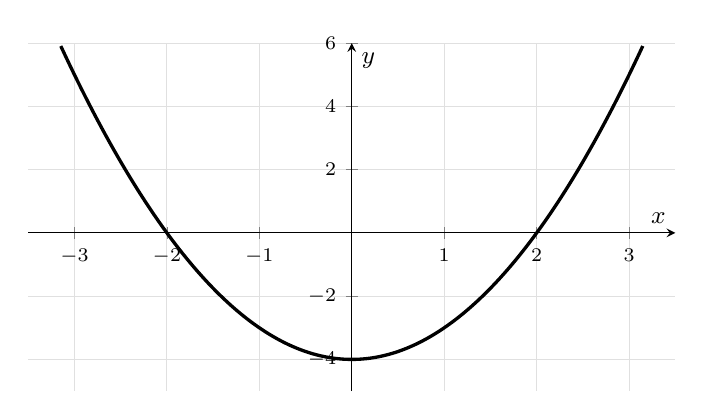
\begin{tikzpicture}
\begin{axis}[
width=9.8cm,height=6cm,axis lines=middle,
xmin=-3.5,xmax=3.5,ymin=-5,ymax=6,
xtick={-3,-2,...,3},ytick={-4,-2,0,2,4,6},grid=both,
minor tick num=0,grid style={black!12},
tick label style={font=\scriptsize},xlabel={$x$},ylabel={$y$},
label style={font=\small},restrict y to domain=-5:6,
clip=true,legend style={font=\scriptsize,draw=none,fill=none,at={(0.98,0.98)},anchor=north east},
]
\addplot[very thick,solid,domain=-3.5:3.5,samples=160] {x^2-4};
\end{axis}
\end{tikzpicture}
\end{center}
\blok{Společně řešené příklady}

\begin{prikladReseniBox}[title={Příklad 1}]
Najděte průsečíky s oběma osami u $f(x)=x^2-4$. Určete vrchol a rozhodněte, kolikrát parabola protne osu $x$.
\tcblower
\[
\begin{aligned}
f(0)&=-4\ \Rightarrow\ P_y[0;-4] \\
x^2-4&=(x-2)(x+2) \\
f(x)=0&\iff x=-2\ \text{nebo}\ x=2 \\
P_{x,1}&[-2;0],\quad P_{x,2}[2;0] \\
V&=[0;-4]
\end{aligned}
\]

\end{prikladReseniBox}
\begin{prikladReseniBox}[title={Příklad 2}]
U funkce $g(x)=x^2-4x+3$ stanovte průsečíky s osami bez použití diskriminantu.
\tcblower
\[
\begin{aligned}
g(0)&=3\ \Rightarrow\ P_y[0;3] \\
x^2-4x+3&=(x-1)(x-3) \\
g(x)=0&\iff x=1\ \text{nebo}\ x=3 \\
P_{x,1}&[1;0],\quad P_{x,2}[3;0]
\end{aligned}
\]

\end{prikladReseniBox}
\begin{prikladReseniBox}[title={Příklad 3}]
Porovnejte $h(x)=(x-2)^2$ a $k(x)=(x+1)^2+4$: kolik mají nulových bodů a proč?
\tcblower
\[
\begin{aligned}
h(x)=0&\iff (x-2)^2=0\iff x=2 \\
k(x)&=(x+1)^2+4\ge4>0 \\
K_h&=\{2\},\qquad K_k=\varnothing
\end{aligned}
\]
První graf se osy $x$ pouze dotýká, druhý leží celý nad ní.
\end{prikladReseniBox}
\blok{Samostatné procvičování}

\begin{zadaniReseniBox}[title={Samostatná práce 1}]
a) Najděte průsečíky s osami u $y=x^2-9$.\par
b) Najděte nulové body $y=-x^2+4x$.\par
c) Rozhodněte, zda $y=-(x-1)^2-2$ protíná osu $x$.
\tcblower
\[
\begin{aligned}
x^2-9&=0\ \Rightarrow\ x=\pm3,\quad P_y[0;-9] \\
-x^2+4x&=x(4-x)=0\ \Rightarrow\ x\in\{0;4\} \\
-(x-1)^2-2&\le-2<0\ \Rightarrow\ \text{žádný nulový bod.}
\end{aligned}
\]

\end{zadaniReseniBox}
\blok{Volitelná rezerva}
Nech žáky z grafu $y=(x-1)^2-4$ nejdřív \emph{odhadnout} kořeny; potom je prověř výpočtem $(x-1)^2=4$. Při dvou řešeních se jeden bod nachází vlevo a druhý vpravo od osy souměrnosti.
\blok{Domácí úkol}
\begin{zadaniReseniBox}[title={Domácí úkol}]
\begin{enumerate}[label=\alph*),itemsep=3pt]
\item U $f(x)=x^2-16$ určete průsečíky s oběma osami.
\item U $g(x)=x^2-5x$ určete nulové body.
\item U $h(x)=(x+3)^2$ určete všechny průsečíky s osou $x$ a osou $y$.
\item Vysvětlete bez rozsáhlého výpočtu, proč funkce $p(x)=x^2+2$ nemá nulový bod.
\item U $q(x)=x^2-2x-3$ určete průsečíky s osami rozkladem.
\item U $r(x)=-(x-1)^2+9$ určete průsečíky s osou $x$ a s osou $y$.
\item \textbf{Výzva:} Rozhodněte počet průsečíků s osou $x$ u $s(x)=2(x+1)^2-3$, určete je přesně.
\end{enumerate}
\tcblower
\begin{enumerate}[label=\alph*),itemsep=4pt]
\item
\[
\begin{aligned}
f(0)&=-16,\quad x^2-16=(x-4)(x+4) \\
P_y&[0;-16],\quad P_{x,1}[-4;0],\ P_{x,2}[4;0]
\end{aligned}
\]

\item
\[
\begin{aligned}
x^2-5x&=x(x-5)=0 \\
K&=\{0;5\}
\end{aligned}
\]

\item
\[
\begin{aligned}
(x+3)^2=0&\iff x=-3 \\
P_x&[-3;0],\qquad P_y[0;9]
\end{aligned}
\]

\item
\[
\begin{aligned}
x^2&\ge0\ \Rightarrow\ x^2+2\ge2>0 \\
K&=\varnothing
\end{aligned}
\]

\item
\[
\begin{aligned}
x^2-2x-3&=(x-3)(x+1) \\
P_{x,1}&[-1;0],\quad P_{x,2}[3;0],\quad P_y[0;-3]
\end{aligned}
\]

\item
\[
\begin{aligned}
(x-1)^2&=9\ \Rightarrow\ x=1\pm3 \\
P_{x,1}&[-2;0],\quad P_{x,2}[4;0] \\
r(0)&=8\ \Rightarrow\ P_y[0;8]
\end{aligned}
\]

\item
\[
\begin{aligned}
2(x+1)^2-3&=0\ \Rightarrow\ (x+1)^2=\tfrac32 \\
x&=-1\pm\sqrt{\tfrac32} \\
\text{Dva body: }&[-1-\sqrt{3/2};0],\ [-1+\sqrt{3/2};0]
\end{aligned}
\]

\end{enumerate}
\end{zadaniReseniBox}
\poznamka{Čas: vysvětlení průsečíků 8 min, první dva příklady 14 min, porovnání počtu kořenů 7 min, samostatně 12 min, závěr 4 min. Nevyvozuj zatím obecný kořenový vzorec; nevyčísluj diskriminant.}
\end{document}
